\chapter{Analýza a implementace klienské části}\label{ch:client}

\chaptersummary{
   \begin{ul}
      \item popis architektury klientské aplikace,
      \item krátký popis potřebných změn na základě předchozí analýzy,
      \item rozbor komplexnějších funkcionalit a aspektů realizace,
      \item rozbor implementace interpretů obsahů na základě analýzy klientských mikroslužeb.
   \end{ul}
}

Klientská část aplikace ve srovnání s původní implementací z konceptuálního pohledu nepotřebuje výrazné zásahy, nebo zněmy.
Vzhledem k zastaralým závislostem projektu budou obnoveny verze knihoven pro dostupnost nových funkcionalit a bude znovu implementován systém interpretování obsahů, který není v současné době dostatečně izolován od prostředí \g{IS}.
Autorizační systém, vzhledem k přechodu na vlastní authentizaci, rovněž bude pozměněn ve větší míře.
Drobné změny klietské implementace nebudou explicitně rozebírány.



\section{Architektura}\label{sec:client-arch}
Po obecném prozkoumání problematiky mikroslužeb na klientské straně v kapitole~\nameref{sec:msa-client} lze udělat závěr, že přechod na mikroslužby u tak omezené aplikace není výhodný – vyváženost komponent se poředpokládá přiměřeně ekvivalentní.
Jediným problémovým místem je realizace interpretů obsahů projketů, u které se předpokládá časté obnovování a dynamické vkládání.

Základ architektury je tudíž převzat z bakalářské práce – řešení založené na frameworku Next.js s využitím \g{SSG} a \g{SSR}.
Obsash projektů i nyní bude tvořen za pomocí načítání externích \h{.js} souborů s vlastní inicializací, ale samotná realizace musí být upravena pro větší izolaci jednotlivých částí obsahu.


\begin{figure}[htbp]
   \centering
   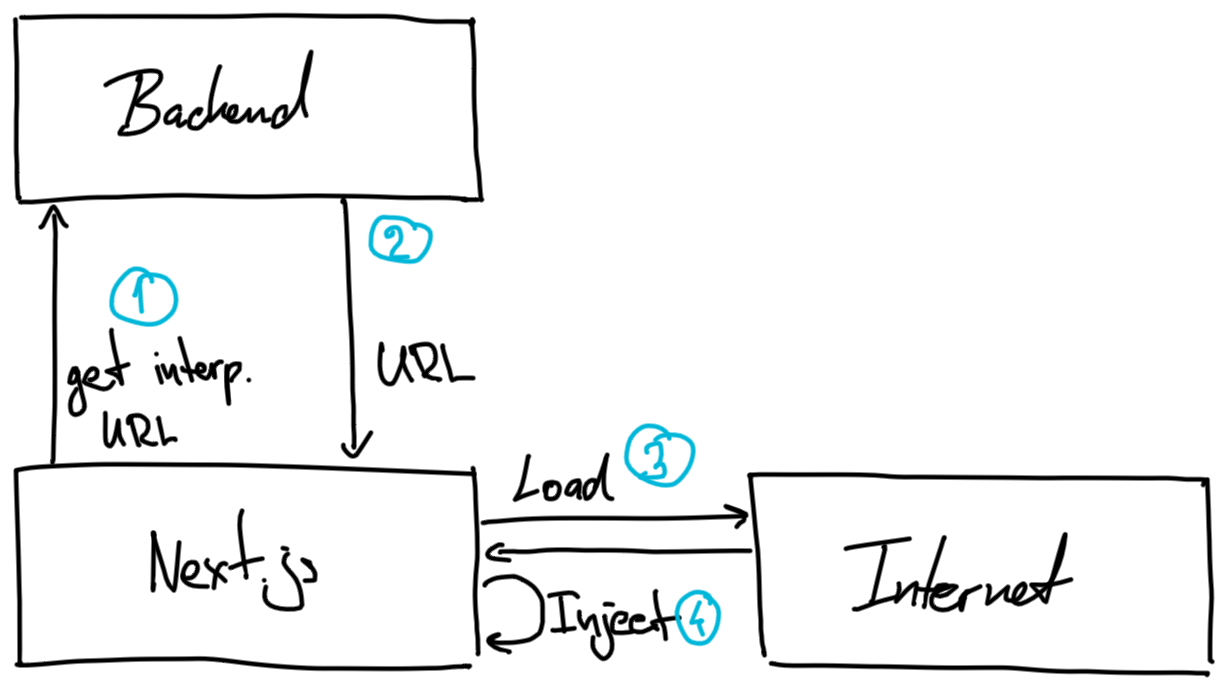
\includegraphics[max width=\textwidth]{assets/draft-fe-arch}
   \caption{Architektura klientské aplikace}\label{fig:client-arch}
\end{figure}



\section{Zdokonalení struktury a funkcionality}\label{sec:client-improve}




\begin{dl}
   \item[Aktualizace závislotí] – Aktualizace vyřešila problémy s instalací vyžadovaných npm balíčků a poskytla nové možnosti pro vývoj.

   \item[Podpora internacionalizace a lokalizace] – V používané knihovně Next.js od verze 10.0.0 je implementována podpora internacionalizace – možnost přidat seznam lokalizovaných prvků a výchozí lokalizaci, o všechny potřebné náležitosti (směrování apod.) se stará knihovna~\cite{nextjsi18n}.
   \TODO{načítání translací z backendu}

   \item[React hooks] –
   Přechod na modernější způsob zápisu React komponent s využitím \enquote{React hooks} nebyl nutný, nicméně v rámci přepisování větší části klietské aplikace bylo rozhodnuto použít nový způsob zápisu.
   Přineslo to (v porovnáním s původním kódem) výrazné snížení objemu kódu a zlepšení přehlednosti.

   Bylo experimentálně ověřeno, že rozdíl z hlediska rychlosti zpracování není tolik výrazný~\cite{reacthooksdiff}.
   Rozdíl se objevuje především v objemu generovaného kódu.
   V případě funkcionální komponenty je objem několikanásobně menší, než v případě class komponenty.

   \item[Nepříznivé scénáře \g{API} dotazů] – Klientské zpracování \g{API} dotazů bylo přepsáno na dotazování s pomocí obalů pro axios knihovnu.
   Obecné chyby se zpracovávají centrálně během přijetí odpovědi ze serveru.
   Chyby závislé na konkrétním dotazu se nyní zpracovávají i vizuálně pro uživatele.

   \item[Vizuální vzhled rozhraní] – vizuální rozhraní bylo upraveno pro lepší \g{UX}.
\end{dl}



\subsection{Autentizace}\label{sec:client-auth}

Větší rozsah změn se dotknul autentizaci a autorizaci uživatele v aplikaci.
Částečně přizpůsobený OAuth 2.0 se nahradil běžnou, nezávislou implementací \enquote{access} a \enquote{refresh} tokenů pro přístup na zabezpečené zdroje.
Zjednodušil se tím postup registrace a přihlašování a eliminoval uživatelky nepříjemný manuální přechod mezi záložkami kvůli synchronizaci dat.
Za veškerou logiku získávání a obnovování tokenů nyní je zodpovědný tzv. \h{axios interceptor}.

\TODO{diagram implementace access a refresh tokenu s pomoci axios}



\section{Interprety obsahu}\label{sec:client-interpret}


\TODO{popsat novou implementaci integrace interpretů}

\begin{figure}[htbp]
   \centering
   
\includegraphics[max width=\textwidth]{assets/draft-interpreters}
   \caption{Způsob tvorby obsahů s pomocí interpretů}\label{fig:client-interpreter}
\end{figure}


V předchozí verzi inplementace byl problém s malou izolovaností výsledku generování obsahu vůči zbytku aplikace.
Vzhledem k systému přímého vkládání nového \h{.js} skriptu do webové stránky úplně izolovat daný proces nejspíš nepůjde, ale je možné ho omezit z několika hledisek:


\begin{dl}
   \item [Izolace \g{CSS}] – během generování nového zdrojového kódu bude hlavní aplikací poskytnut unikátní \g{ID} části obsahu, který se použije jako prefix všech \g{CSS} pravidel.
   Tím se zajistí, že styly budou uzavřeny ve vlastním \g{DOM} uzlu.
   Vzhledem k dostupným \g{CSS} selektorům to nezabrání úmyslnému upravování stylů vně části obsahu, ale zamezí to nechtěnným modifikacím v jiných částech aplikace.
   \item [Izolace \g{JS}] – do globální úrovně proměnných se bude muset stále přistupovat, ale samotný interpet může běže nezávisle ve vlastním kontextu.
   Toto chování již bylo realizováno a nemění se.
\end{dl}
